%% Road to VPhO 2023 Template

\documentclass[12pt]{article}
\usepackage[english]{babel}
\usepackage[T5]{fontenc}
\usepackage[top=2cm, bottom=2cm, left=2cm,right=2cm]{geometry} %%%% Margin %%%%%
\usepackage[dvipsnames]{xcolor}
\usepackage[pdftex]{graphicx}
\usepackage{wrapfig}
\usepackage{tcolorbox}
\usepackage{mathtools}
\usepackage{amsmath}
\usepackage{amssymb}
\usepackage{eqnarray}
\usepackage{siunitx}
\usepackage{array, lipsum, bibentry,fancyhdr}
\usepackage{hyperref}
\usepackage{natbib}
\setlength{\parindent}{0pt}
\usepackage{enumitem}
\usepackage[noframe]{showframe}
\usepackage{framed}
\usepackage{titling}
\usepackage{float}
\usepackage{multicol}
\usepackage{url}
\usepackage{authblk}
\usepackage{sectsty}
\usepackage{eqparbox}

%%%%%%%%%% Pictures drawing %%%%%%%%%%%%%

\usepackage{pgfplots} %%%%%% Regression %%%%
\pgfplotsset{compat = newest}
\usepackage{pgfplotstable}
\usepackage{tikz}
\usepackage{tikz-3dplot} %%%%%% Draw %%%%%%
\usepackage{tikz,tkz-euclide}
\usetikzlibrary{arrows,calc,patterns}
\usetikzlibrary{quotes,angles}
\usetikzlibrary{shapes.geometric}
\usepackage{circuitikz} %%%%% Circuit %%%%
\usetikzlibrary{decorations.pathmorphing,patterns}

\setlength{\unitlength}{1cm}

%%%%%%%%%% Hyperlink %%%%%%%%%%%%%

\hypersetup{
	colorlinks=true,
	linkcolor=black,
	filecolor=mangeta,      
	urlcolor=blue,
	pdftitle={Overleaf Example},
	pdfpagemode=FullScreen,
}

%%%%%%%%%% Header & Footer %%%%%%%%%%%%%

\setlength{\headheight}{10mm}
\RequirePackage{fancyhdr}  % Needed to define custom headers/footers
\RequirePackage{lastpage}  % Number of pages in the document
\pagestyle{fancy}          % Enables the custom headers/footers
% Headers
\lhead{
\includegraphics[width=.8in]{xPhO.png}}%
\chead{}%
\rhead{\small\sffamily\bfseries{Đề bài hướng tới VPhO 42} --- \thepage/\pageref{LastPage}}
% Footers
\lfoot{}%
\cfoot{}%
\rfoot{}%
\renewcommand{\headrulewidth}{1pt}% % header rule
\renewcommand{\footrulewidth}{1pt}% % footer rule

% \pagestyle{fancy}
% 	\fancyhead[L]{\empty}
% 	\fancyhead[R]{\empty}
% 	\fancyhead[C]{\empty}
% 	\fancyfoot[C]{\empty}
% 	\fancyfoot[L]{\empty}
% 	\renewcommand{\headrulewidth}{0pt}
% 	\fancyfoot[C]{\normalcolor{\thepage/\pageref{LastPage}}}
% 	\setcounter{page}{1}

%%%%%%%%%% Color setup %%%%%%%%%%%%%

\RequirePackage{xcolor}
\definecolor{wsdred}{HTML}{8E1728}
\definecolor{wsdgrey}{HTML}{75787B}
\renewcommand{\normalcolor}{\color{wsdred}}
\colorlet{ColorOr}{white}

\begin{document}

%% Title %%
{\fontsize{50}{24}\fontfamily{phv}\fontseries{b}
\LARGE \normalcolor{Đề bài hướng tới VPhO 42} }

\textcolor{blue}{\textbf{\textit{Câu lạc bộ vật lý xPhO}}}

%%%%
\vspace{5mm}

{\normalcolor\textbf{CÂU 1. (4.0 điểm)}}\vspace{1.5mm}

\setcounter{equation}{0}
Một quả lựu đạn đang đứng yên ở độ cao $H$ so với mặt đất thì phát nổ và bắn ra các mảnh đạn giống nhau với cùng tốc độ $v_0$, phân bố các mảnh đạn khi văng ra là đẳng hướng. Gia tốc trọng trường là $\Vec{g}$.
\begin{enumerate}[label=\textbf{\alph*,}]\itemsep0em
    \item Xác định phương trình mặt cong ba chiều biểu diễn ranh giới giữa \textit{vùng an toàn} và \textit{vùng nguy hiểm}, tức là trong vùng an toàn thì mảnh đạn sẽ không thể bay tới, ngược lại với vùng nguy hiểm. Vẽ phác dạng đồ thị của đường ranh giới, ghi chú thích và các điểm đặc biệt.
    \item Sau khi các mảnh đạn rơi hết xuống đất, xác định bán kính $R$ của vùng đạn đã rơi trên mặt đất.
    \item Giả sử rằng lựu đạn chứa $M$ khối lượng đạn nổ trong một góc nón nhỏ hướng lên trên với góc mở $2\alpha_0 \ll 1$, bom nổ trên mặt đất ($H = 0$). Chứng minh rằng phân bố khối lượng mặt $\rho(r)$ (khai triển tới thành phần bậc hai $r^2$) của đạn trên mặt đất khi tất cả mảnh đạn đã rơi xuống đất có dạng như sau
    $$\rho(r) \approx \rho_0 (1 + \beta r^2),$$

    hãy biểu diễn $\rho_0$ và $\beta$ theo các thông số đã biết.
\end{enumerate}

\textit{Có thể sử dụng xấp xỉ sau:} $\displaystyle \sin \alpha \approx \alpha \left(1 - \frac{1}{6} \alpha^2 \right)$.

\begin{flushright}
    (Biên soạn bởi Zinc)
\end{flushright}

{\normalcolor \textbf{CÂU 2. (4.0 điểm)}}\vspace{1.5mm}

\setcounter{equation}{0}
\textbf{Chu trình dưới tới hạn cho máy lạnh}\\

Carbon dioxide (\(\mathrm{CO}_2\)) đã từng được sử dụng phổ biến trong các loại máy lạnh và điều hòa vào cuối thế kỉ XIX và đầu thế kỉ XX, trước khi các loại khí ga làm lạnh tổng hợp được phát minh. Trong những năm trở lại đây, khi người ta quan tâm hơn về ảnh hưởng môi trường của các loại ga làm lạnh đang được sử dụng phổ biến, carbon dioxide đang trở lại như một lựa chọn tiềm năng với tác động môi trường thấp, không độc, rẻ và có sẵn, và với những đặc tính nhiệt động và thủy động học có lợi cho thiết kế các hệ thống điều hòa. \\

Chúng ta sẽ cùng khảo sát hoạt động của một hệ thống điều hòa thông dụng ở chế độ dưới bão hòa: Cho \(n\) mol của một loại khí ga thực hiện chu trình như được miêu tả trên đồ thị 1a và 1b, với \(h\) và \(s\) lần lượt là enthalpy và entropy riêng của 1 mol. Lưu ý: hình vẽ không theo tỉ lệ. \\

\begin{center}
    \begin{tikzpicture}
%Đồ thị p-h
  \draw[->] (0,0) -- (6,0) node[below] {$h$};
  
  \draw[->] (0,0) -- (0,4) node[left] {$p$};
  \draw (3,1.5) -- (4.5,3) -- (1,3) -- (1,1.5) -- (3,1.5);
  \draw [dashed] (1,3) -- (0,3);
  \draw [dashed] (1,1.5) -- (0,1.5);
  \filldraw[black] (4,3) circle (1pt);
  \node at (3,1.2) {1};
  \node at (4.5,3.2) {2};
  \node at (4,3.2) {3};
  \node at (1,3.2) {4};
  \node at (1,1.2) {5};
  \node at (-0.3,-0.3) {O};
  \node at (-0.7,3) {$p_{bh}(T_H)$};
  \node at (-0.7,1.5) {$p_{bh}(T_C)$};
    \node at (3,-1) {\textbf{(a)}};
%Đồ thị T-s 
  \draw[->] (8,0) -- (14,0) node[below] {$s$};
  \draw[->] (8,0) -- (8,4) node[left] {$T$};
  \draw (12.5, 1.5) -- (12.5, 3.5);
  \draw plot [smooth, tension = 2] coordinates{(12.5, 3.5) (12.3, 3.2) (12, 3)};
  \draw (12, 3) -- (9,3);
  \draw [dashed] (9,3) -- (10,1.5);
  \draw (10,1.5) -- (12.5,1.5);
  \draw [dashed] (9,3) -- (8,3);
  \draw [dashed] (10,1.5) -- (8,1.5);
  \node at (7.7,-0.3) {O};
  \node at (12.5, 1.2) {1};
  \node at (12.5, 3.7) {2};
  \node at (12, 3.2) {3};
  \node at (9, 3.2) {4};
  \node at (10, 1.2) {5};
  \node at (7.7, 3) {$T_H$};
  \node at (7.7,1.5) {$T_C$};
  \node at (11,-1) {\textbf{(b)}};
\end{tikzpicture} \\
Hình 1: \textbf{(a)} Giản đồ $p-h$ của khí ga. \textbf{(b)} Giản đồ $T-s$ của khí ga.
\end{center}
Chu trình này được mô tả như sau: \\
1-2: Nén khí đoạn nhiệt \\
2-3: Làm mát đẳng áp \\
3-4: Ngưng tụ đẳng nhiệt \\
4-5: Giãn khí đột ngột (Quá trình Joule - Thompson) \\
5-1: Bay hơi đẳng nhiệt \\

Áp suất hơi bão hòa tại nhiệt độ \(T_H\), \(T_C\), enthalpy riêng của pha lỏng, nhiệt hóa hơi mol của pha lỏng coi như đã biết. Giả sử rằng ở thể hơi, khí ga này là một khí lý tưởng đa nguyên tử.
\begin{enumerate}
    \item Tìm nhiệt độ \(T_2\) theo \(T_C\), \(p_{bh}(T_C)\), \(p_{bh}(T_H)\).
    \item Tìm nhiệt lượng do ga tỏa ra trong quá trình 2-3 và 3-4.
    \item Quá trình giãn khí là một quá trình xảy ra rất nhanh, khi đó ta có thể bỏ qua sự trao đổi nhiệt của ga với môi trường trong quá trình này. Thừa nhận rằng tổng enthalpy của ga không đổi trong quá trình này. Tìm tỉ lệ mol ga bị hóa hơi ở cuối quá trình 4-5.
    \item Tìm nhiệt lượng khí ga thu vào trong quá trình 5-1.
    \item Tìm công cần cung cấp cho ga để thực hiện một chu trình theo \(T_h\), \(T_c\), \(p_{bh}(T_h)\), \(p_{bh}(T_c)\), \(h(T_H)\), \(h(T_C)\).
    \item Tìm hiệu suất của chu trình.
    \item Áp dụng số cho \(\mathrm{CO}_2\) với \(T_H = \SI{20}{^{\circ} C}\) và \(T_C = \SI{0}{^{\circ} C}\), nhiệt hóa hơi \(L = \SI{16.5}{kJ/mol}\). Vì sao chu trình này với ga \(\mathrm{CO}_2\) lại không được dùng cho điều hòa nhiệt độ tại nhà thông thường?.
\end{enumerate}

% \vspace{3mm}
% Bảng 1: Các thông số nhiệt động lực học của pha lỏng của \(\mathrm{CO}_2\) tại áp suất hơi bão hòa theo nhiệt độ
% \begin{figure}[H]
%     \centering
%     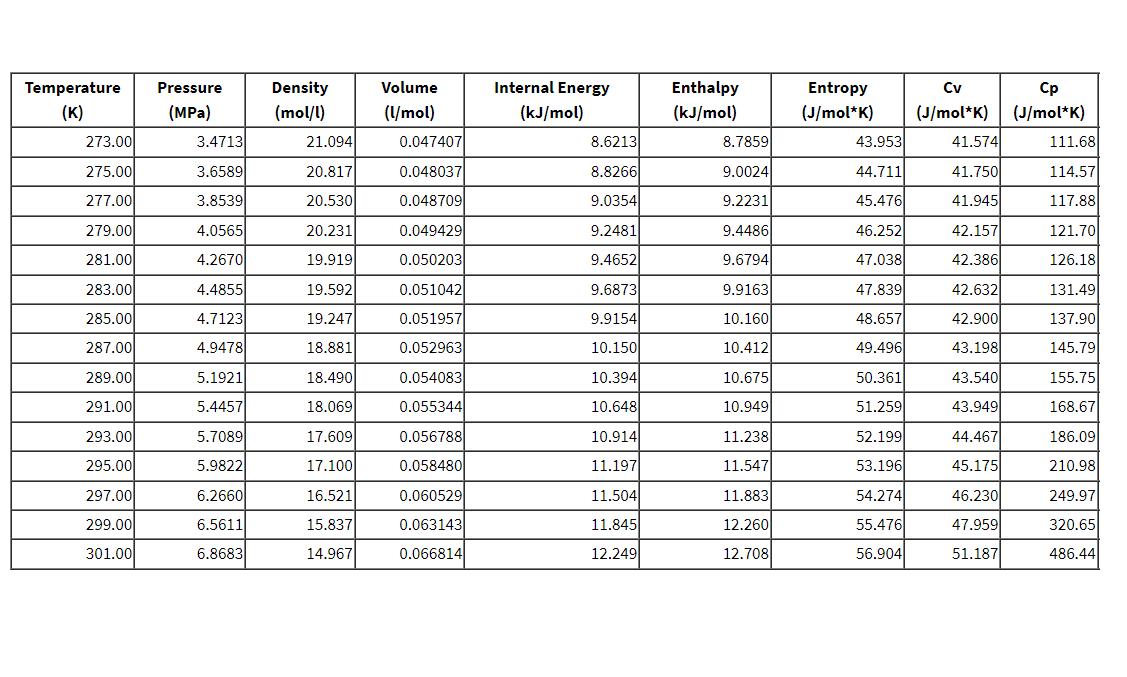
\includegraphics[scale=0.75]{Problem_2/Liquid_phase.png}
    
%     \label{fig:enter-label}
% \end{figure}

\begin{center}
\footnotesize{
\begin{tabular}{|>{\centering\arraybackslash}m{2cm}|>{\centering\arraybackslash}m{2cm}|>{\centering\arraybackslash}m{2cm}|>{\centering\arraybackslash}m{2cm}|>{\centering\arraybackslash}m{2cm}|>{\centering\arraybackslash}m{2cm}|}
    \hline
    Nhiệt độ & Áp suất & Mật độ mol & Nội năng & Enthalpy & Entropy \\
    $(\si{K})$ & $(\si{MPa})$ & $(\si{mol/l})$ & $(\si{kJ/mol})$ & $(\si{J/mol \cdot K})$ & $(\si{J/mol \cdot K})$ \\
    \hline
    273.00 & 3.4713 & 21.094 & 8.6213 & 8.7859 & 43.953 \\
    \hline
    275.00 & 3.6589 & 20.817 & 8.8266 & 9.0024 & 44.711 \\
    \hline
    277.00 & 3.8539 & 20.530 & 9.0354 & 9.2231 & 45.476 \\
    \hline
    279.00 & 4.0565 & 20.231 & 9.2481 & 9.4486 & 46.252 \\
    \hline
    281.00 & 4.2670 & 19.919 & 9.4652 & 9.6794 & 47.038 \\
    \hline
    283.00 & 4.4855 & 19.592 & 9.6873 & 9.9163 & 47.839 \\
    \hline
    285.00 & 4.7123 & 19.247 & 9.9154 & 10.160 & 48.657 \\
    \hline
    287.00 & 4.9478 & 18.881 & 10.150 & 10.412 & 49.496 \\
    \hline
    289.00 & 5.2921 & 18.490 & 10.394 & 10.675 & 50.361 \\
    \hline
    291.00 & 5.4457 & 18.069 & 10.648 & 10.949 & 51.259 \\
    \hline
    293.00 & 5.7089 & 17.609 & 10.914 & 11.238 & 52.199 \\
    \hline
    295.00 & 5.9822 & 17.100 & 11.197 & 11.547 & 53.196 \\
    \hline
    297.00 & 6.2660 & 16.521 & 11.504 & 11.883 & 54.274 \\
    \hline
    299.00 & 6.5611 & 15.837 & 11.845 & 12.260 & 55.476 \\
    \hline
    301.00 & 6.8683 & 14.967 & 12.249 & 12.708 & 56.904 \\
    \hline
\end{tabular}
}
\end{center}

\begin{flushright}
    (Biên soạn bởi Yuki)
\end{flushright}

{\normalcolor \textbf{CÂU 3. (4.0 điểm)}}\vspace{1.5mm}

\setcounter{equation}{0}
% \textbf{Định lý Earnshaw và thấu kính tĩnh điện}

% Một vòng dây điện tích \(Q\) hình đa giác đều \(n\) cạnh có bán kính đường tròn ngoại tiếp \(R\). Trục \(\Delta\) là trục đi qua tâm và vuông góc với mặt phẳng vòng dây có dạng đối xứng trụ.

% \ \ 

% \textbf{1.} Chứng minh rằng, điện trường ở gần trục \(\Delta\).

% \ \ 

% \textbf{2.} Tính vector điện trường \(\mathbf{E}\) tại một vị trí gần trục \(\Delta\).

% \ \ 

% Theo định lý Earnshaw, một hệ điện tích trong chân không không thể tạo ra một điểm cân bằng bền chỉ bởi các tương tác tĩnh điện.

% \ \  

% \textbf{3.} Chỉ ra rằng trong bài toán này, vị trí cân bằng không thể là vị trí cân bằng bền với mọi chuyển động.

% \ \ 

% \textbf{4.} Bắn một hạt điện tích \(q\) khối lượng \(m\) với vận tốc \(v_0\) song song với trục \(\Delta\) và cách trục \(\Delta\) một khoảng \(b\) (với \(b \ll R\) ). Quỹ đạo của hạt điện tích đi qua vòng dây điện tích giống như một tia sáng đi qua thấu kính có tiêu cự \(f\). Tính tiêu cự \(f\) này theo \(n\), \(R\), \(Q\), \(q\), \(\varepsilon_0\), \(m\) và \(v_0\).

\textbf{Hiệu ứng bề mặt} \footnote{Skin effect.}

Hiệu ứng bề mặt là một hiệu ứng xuất hiện phổ biến trong các các đường mạch điện truyền dẫn dòng điện cao tần. Theo đó, thay vì phân bố đều trên toàn dây dẫn như các dòng điện tần số thấp, ở tần số cao, các dòng điện tập trung chủ yếu ở sát bề mặt kim loại và nhanh chóng giảm theo độ sâu với cấp số mũ.

\ \

\textbf{1. Mô hình mạch tương đương đơn giản}

Quy luật chuyển động của dòng điện trong một vật dẫn với hằng số điện môi \(\mu\) và điện trở suất \(\rho\) có thể được mô tả bởi một mạch điện tương đương (như hình \ref{fig:Equivalent_circuit_skin_effect}) \footnote{Điện kháng \(L_0\) được sử dụng để mô tả hằng số từ thẩm trong chân không \(\mu_0\) của môi trường ngoài. Ta không cần quan tâm đến nó trong bài toán này}. Ở hình \ref{fig:Equivalent_circuit_skin_effect}A, phân bố dòng điện trong tấm vật liệu được tương đương như một mạch điện vô hạn, theo đó, từng khối chữ nhật có chiều dài \(l\), chiều rộng \(w\) và độ dày \(\Delta z\) (như hình \ref{fig:Conductor}) được tương đương như một mắt mạch tương đương gồm một thành phần cảm kháng \(\Delta L\) và một phần điện dẫn \footnote{Nghịch đảo của điện trở.} \( \Delta G \).

\begin{figure}[!h]
    \centering
    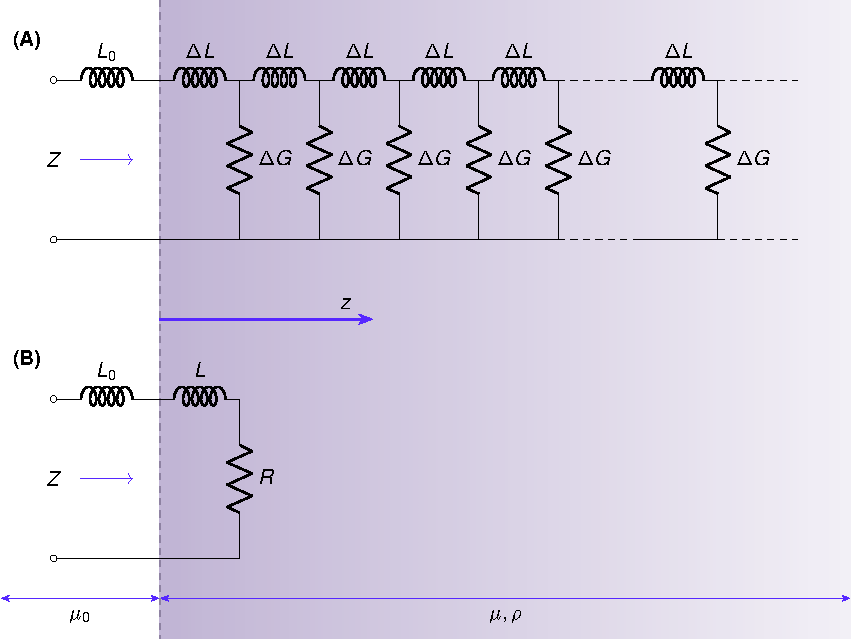
\includegraphics[width=0.9\textwidth]{Problem_3/Figs_P3/Equivalent_circuit_skin_effect.pdf}
    \caption{Mô hình mạch tương đương của hiệu ứng bề mặt. (A) Mạch tương đương phân bố vô hạn trong không gian. (B) Mạch tương đương trở kháng của mạch.}
    \label{fig:Equivalent_circuit_skin_effect}
\end{figure}

Dựa vào các tính toán mạch tương đương, mạng mạch vô hạn tuần hoàn trên có trở kháng quan sát từ phía bề mặt ngăn cách hai môi trường là \(Z\) và có thể được phân tích như tổng của hai phân tử \(R\) và \(L\) (như hình \ref{fig:Equivalent_circuit_skin_effect}B).

\begin{figure}
    \centering
    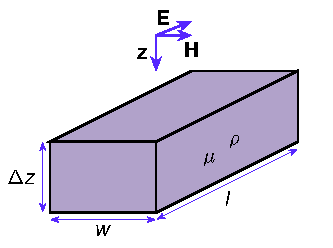
\includegraphics[width=0.6\textwidth]{Problem_3/Figs_P3/Conductor.pdf}
    \caption{Mô hình một phần tử trong khối vật dẫn.}
    \label{fig:Conductor}
\end{figure}

\textbf{Câu hỏi a.} Tìm \( \Delta L \) và \( \Delta G \) của mạch trong mô hình mạch tương đương vô hạn theo \(\mu\), \(\rho\), \(w\), \(l\) và \( \Delta z \).

\ \

\textbf{Câu hỏi b.} Tìm các thông số trở kháng \(Z\), \(R\) và \(L\) theo \(\mu\), \(\rho\), \(w\), \(l\) và tần số \(\omega\) của dòng điện.

\ \

\textbf{Câu hỏi c.} Độ sâu bề mặt\footnote{Skin depth.} là độ sâu để biên độ dòng điện giảm đi \(e\) lần. Xác định độ sâu bề mặt của tấm vật liệu theo tần số \(\omega\) của dòng điện, độ từ thẩm \(\mu\) và điện trở suất \(\rho\).

\ \

\textbf{2. Điện trở gây bởi hiệu ứng bề mặt}

\ \

\textbf{Câu hỏi d.} Chứng minh rằng, ta có thể tính điện trở \(R\) tương đương của một đoạn vật dẫn điện chịu ảnh hưởng bởi hiệu ứng bề mặt có thể tính theo công thức:
\begin{equation}
    R = \dfrac{1}{\mu_0} \dfrac{\partial L_0}{\partial z} R_S,
\end{equation}
trong đó
\begin{itemize}
    \item \(L_0\) là độ tự cảm của một miếng bề mặt vật dẫn được xét với giả thiết độ sâu bề mặt bằng không.
    \item Tọa độ \(z\) được hiểu là tọa độ có trục vuông góc với bề mặt.
    \item \(R_S = \sqrt{\omega \mu \rho/2}\) được gọi là hệ số điện trở suất bề mặt.
\end{itemize}

\ \

\textbf{Câu hỏi e.} Tính điện trở gây ra bởi hiệu ứng bề mặt đối với hai ống dây dẫn tròn có chiều dài \(l\), bán kính \(a\) và có trục dây đặt cách nhau một khoảng \(2b\).

{\normalcolor\textbf{CÂU 4. (4.0 điểm)}}\vspace{1.5mm}

\setcounter{equation}{0}
\textbf{Khuếch đại thuật toán}

Bộ khuếch đại thuật toán (OPerational AMPlifier), hay còn gọi là OPAMP là một linh kiện điện tử dùng để thực hiện một số phép toán như cộng, trừ, nhân, chia, tích phân, đạo hàm,... khi nó kết hợp với các linh kiện bên ngoài.

Một OPAMP cơ bản có cấu tạo gồm 8 chân, nhưng trong khuôn khổ bài này, chúng ta chỉ xét một OPAMP như hình vẽ


\begin{figure}[h]
\centering
\begin{subfigure}[t]{0.3\textwidth}
\centering
\begin{circuitikz} 
    \draw
     (0,0) node[op amp] (opamp) {}
     (opamp.+) node[left] {$v_+$}
     (opamp.-) node[left] {$v_-$}
     (opamp.out) node[right] {$v_o$}
     (opamp.up) --++(0,0.5) node[vcc]{$V_+$}
     (opamp.down) --++(0,-0.5) node[vee]{$V_-$};
    \end{circuitikz}
 \caption{Ký hiệu OPAMP}
 \end{subfigure}
 %
\begin{subfigure}[t]{0.6\textwidth}
 \centering
 \begin{circuitikz}[american,scale=0.73,font=\footnotesize]
 \ctikzset{bipoles/length=11mm} 
    \draw
        (0,4) to[short, -o] ++(-1.7,0) node[shift={(-0.4,0)}] {$v_-$}
        (-1.7, 3.6) to [short, -*] (-1.7, 3.6) node[ground]{}
        (0,0) to[short, -o] ++(-1.7,0) node[shift={(-0.4,0)}] {$v_+$}
        (-1.7,-0.4) to [short, -*] (-1.7,-0.4) node[ground]{}
        (0,4) to[resistor, l=$R_\text{in}$] (0,0)
        (1.5,0.5) to [short,-*] (1.5,0.5) node[ground]{} to [cV, invert, l_=$A(v_+ - v_-)$] ++(0,1.5) to [resistor, l=$R_\text{out}$] ++(5.5,0) to [short, -o] ++(0.1,0) node[shift={(0.4,0)}] {$v_\text{o}$}
        (-1,-2) to [short] ++(0,8) to [short] (6.5,2) to [short] (-1,-2) 
        (-1.7, 3) node[below,shift={(-0.,0)} ] {$v_G=0$}
    ;\end{circuitikz}
 \caption{Mạch tương đương của OPAMP}\label{opampcircuit}
 \end{subfigure}
 \caption{OPAMP}
 \end{figure}


Trong đó hai chân $V_+$ và $V_-$ dùng để cấp nguồn cho thiết bị, khi có hai điện thế $v_+$ và $v_-$ được đặt lần lượt vào hai đầu vào không đảo ngược và đảo ngược thì ở đầu ra sẽ xuất hiện một điện thế $v_0$ sao cho:
\begin{equation}
    v_0=A(v_+-v_-) \ \ ,
\end{equation}
trong đó A được gọi là "độ lợi vòng lặp hở" đặc trưng với từng loại OPAMP. Thiết bị này có thể được miêu tả bằng mô hình mạch điện \subref{opampcircuit}, trong đó ký hiệu của nguồn $A(v_+ - v_-)$ gọi là nguồn áp phụ thuộc, tức là độ lớn của nó phụ thuộc vào một đại lượng khác(ở đây là hiệu điện thế giữa hai đầu vào của OPAMP). 




Trong thực tế, OPAMP thường được kết hợp với một số linh kiện ngoài như điện trở, tụ điện hoặc cuộn cảm để phản hồi giữa đầu ra và đầu vào, giúp cho chúng ta có thể điều chỉnh được độ lợi của OPAMP bằng cách điều chỉnh các thông số thiết bị ngoài.
\begin{enumerate}
    \item Tìm độ lợi vòng lặp đóng $\dfrac{v_\text{o}}{v_\text{s}}$ cho mạch dưới đây. Áp dụng với LM741 có độ lợi vòng lặp mở $2 \times 10^5$, điện trở đầu vào $2 \si{M\Omega}$ và điện trở đầu ra $50 \si{\Omega}$ và $R_f=200 \si{\Omega}$, $R_1=100 \si{\Omega}$.
\end{enumerate}
\begin{center}
    \begin{circuitikz}[american]\draw
(0,0) node[op amp] (opamp) {}
 (opamp.+)  to [short] ++ (-1.5,0) to [short] ++(0,-2) node[ground]{} 
 (opamp.-) to [R,l_={$R_1$},i_<=$i_1$] ++(-3,0) to [V, l_=$v_\text{s}$] ++(0,-3) to [short,-o] ++(6,0) node[right]{$-$}
 (opamp.out) to [short,-o] ++(0.62,0) node[right] {$+$}
 (1.64,-1.3) node[right]{$v_o$}
 (opamp.-) to [short]++(-0.5,0) to [short] ++(0,1) to [R,l={$R_f$},i>=$i_f$] ++(2.9,0) to (opamp.out)
 (opamp.-) node[above left]{I}
 (opamp.out) node[above right]{O}
;\end{circuitikz}
\end{center}

Tiếp theo đây, để cho đơn giản, ta coi các OPAMP là lý tưởng, nghĩa là điện trở đầu vào rất lớn, điện trở đầu ra rất nhỏ và độ lợi vòng lặp hở rất lớn. Khi đó $v_1 \approx v_2$ và dòng điện ở hai đầu vào OPAMP $i_-=i_+=0$.
\begin{enumerate}[resume]
    \item Tìm tỉ số $\dfrac{v_o}{v_s}$ với mạch trên khi OPAMP là lý tưởng.    
\end{enumerate}
Xét ba mạch OPAMP có dạng như hình vẽ:
\begin{figure}[h]
\begin{subfigure}[t]{0.6\textwidth}
\centering
\begin{circuitikz}[american,scale=1]
\draw
(-2,0) node[op amp] (opamp) {}
 (opamp.+) to [short] ++ (-1.5,0) to [short] ++(0,-2) node[ground]{} 
 (opamp.-) to [short] ++(-4.5,0) to[R,l_={$R_2$}] ++(0,-1.5)to [V, l_=$v_\text{2}$] ++(0,-1.5)
 (opamp.-) to [short] ++(-3,0) to[R,l_={$R_1$}] ++(0,-1.5)to [V, l_=$v_\text{1}$] ++(0,-1.5)
 (opamp.-) to [short] ++(-6,0) to[R,l_={$R_3$}] ++(0,-1.5)to [V, l_=$v_\text{3}$] ++(0,-1.5) to [short,-o] ++(9,0) node[right]{$-$}
 (opamp.out) to [short,-o] ++(0.62,0) node[right] {$+$}
 (-0.5,-1.3) node[]{$v_\text{sum}$}
 (opamp.-) to [short] ++(0,1) to [R,l={$R_f$},i>=$i_f$] ++(2.4,0) to (opamp.out)
;\end{circuitikz}
 \caption{Mạch cộng}
 \end{subfigure}
 %
\begin{subfigure}[t]{0.4\textwidth}
 \centering
 \begin{circuitikz}[american,font=\small]\draw
(0,0) node[op amp] (opamp) {}
 (opamp.+) to [short] ++ (-1.5,0) to [V,l=$v_s$] ++(0,-2) node[ground]{} 
 (opamp.-) to [R,l_={$R$}] ++(-3,0) to [short] ++(0,-3) to [short,-o] ++(6,0) node[right]{$-$}
 (opamp.out) to [short,-o] ++(0.62,0) node[right] {$+$}
 (1.64,-1.3) node[right]{$v_\text{ni}$}
 (opamp.-) to [short] ++(0,1) to [R,l={$R_f$},i>=$i_f$] ++(2.4,0) to (opamp.out)
 ;\end{circuitikz}
 \caption{Mạch khuếch đại không đảo}
 \end{subfigure}\\[1ex]
\begin{subfigure}{\linewidth}  
\centering
 \begin{circuitikz}[american]\draw
(0,0) node[op amp] (opamp) {}
 (opamp.+) to [short] ++ (-1.5,0) to [short] ++(0,-2) node[ground]{} 
 (opamp.-) to [R,l_={$R$}] ++(-3,0) to [V, l=$v_\text{s}$] ++(0,-3) to [short,-o] ++(6,0) node[right]{$-$}
 (opamp.out) to [short,-o] ++(0.62,0) node[right] {$+$}
 (1.64,-1.3) node[right]{$v_\text{int}$}
 (opamp.-) to [short] ++(0,1) to [C,l={$C$},i>=$i_f$] ++(2.4,0) to (opamp.out)
  ;\end{circuitikz}
 \caption{Mạch tích phân}
 \end{subfigure}
 \end{figure}

\begin{enumerate}[resume]
    \item Tìm $v_\text{sum}$ ,$v_\text{int}$ và $v_\text{ni}$ ứng với ba mạch.
    \item Từ các mạch trên, thiết lập mạch điện để giải phương trình vi phân sau:
    \begin{equation}
        a\dfrac{d^2x}{dt^2}+b\dfrac{dx}{dt}+cx=d ,
    \end{equation}
với điều kiện ban đầu $\dot{x}(0)=e$, $x(0)=f$ .
    \item Đề xuất một cách thiết kế để tạo ra một phần tử mạch điện có giá trị "điện trở âm" ($V_{in}/I_{in} < 0$) bằng các điện trở, OPAMP và nối đất.  
\end{enumerate}

\begin{flushright}
    (Biên soạn bởi Hiagari)
\end{flushright}



{\normalcolor\textbf{CÂU 5. (4.0 điểm)}}\vspace{1.5mm}

\setcounter{equation}{0}
\textbf{Nguyên lý Cực đại Entropy và Đàn chim Bay}

Vật lý hiện diện trong thế giới quanh ta, giúp mô tả các hành vi quần thể của những hệ thống tương tác phức tạp, từ đám khí lý tưởng đến đám đông người. Trong bài tập này, chúng ta sẽ cùng khám phá xem nguyên lý cực đại entropy đã được áp dụng như thế nào để thành lập lên một trong những lý thuyết Vật Lý Sinh thành công nhất hiện đại dùng để mô tả đàn chim bay (xem hình \ref{fig:Bird}A).

\begin{figure}[!h]
    \centering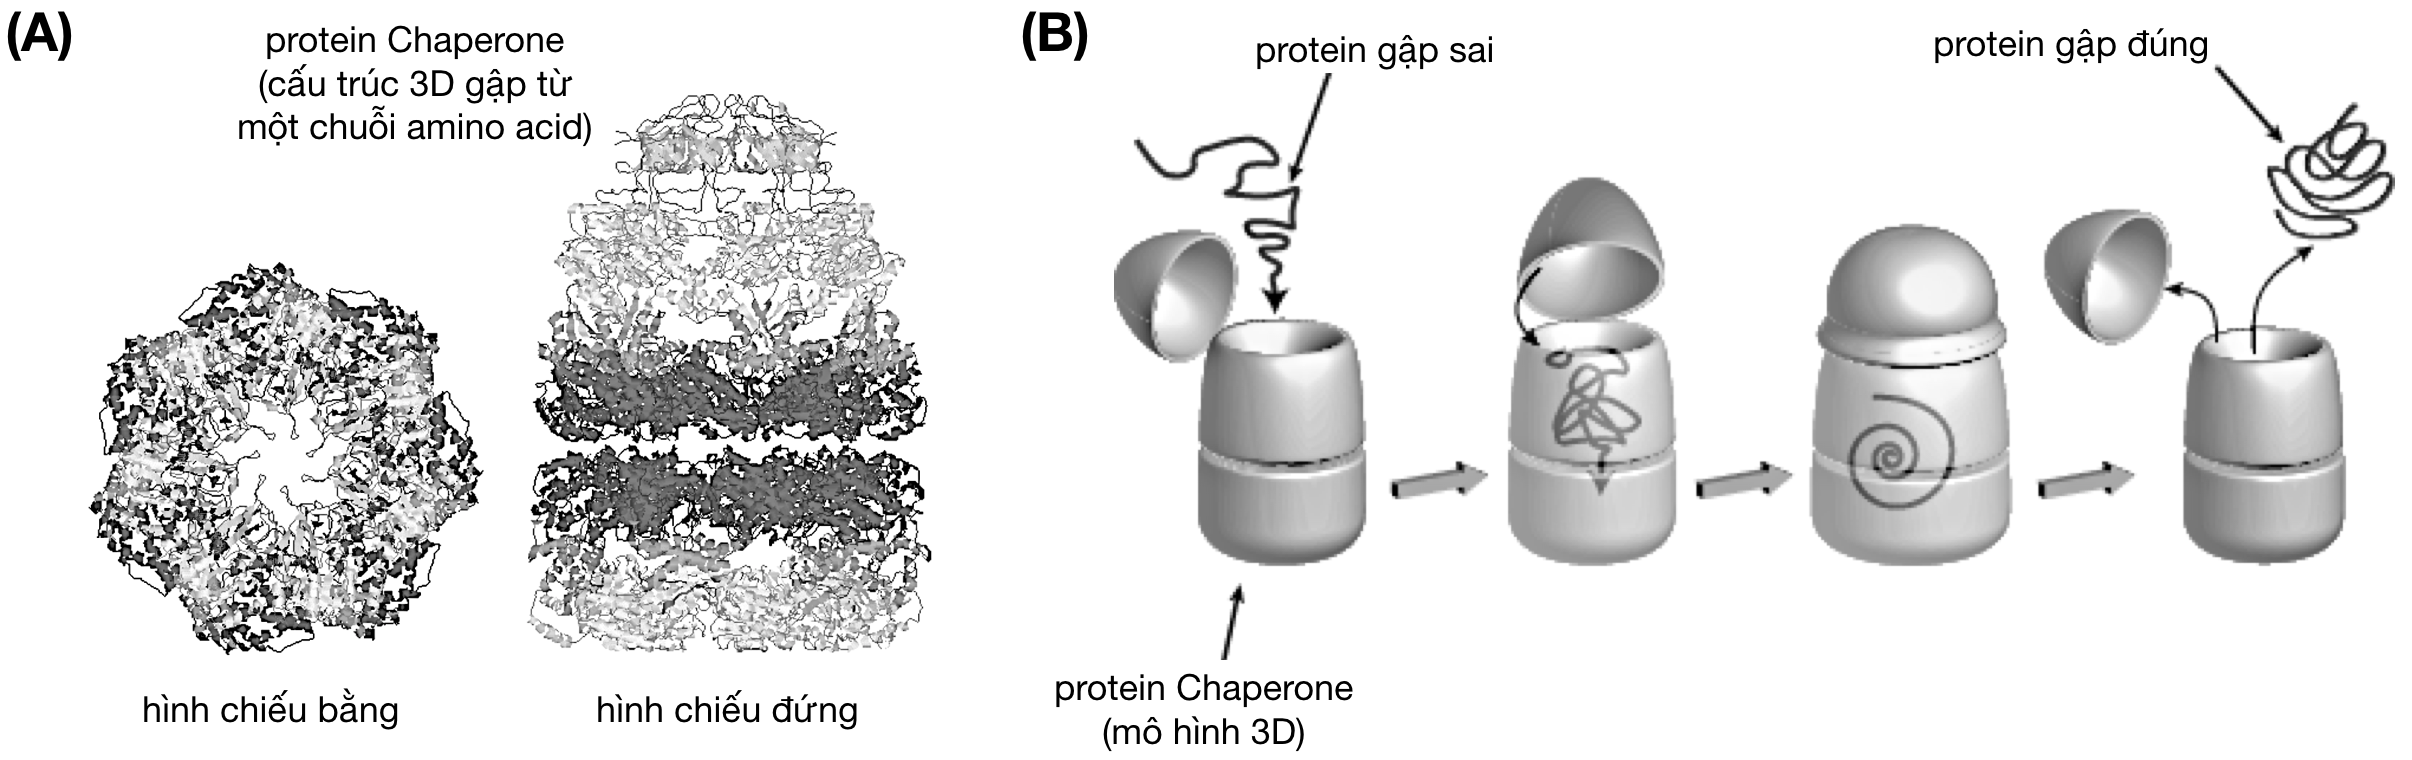
\includegraphics[width=0.96\textwidth]{Problem_5/Figs_P5/fig01.png}
    \caption{(A) Đàn chim bay. (B) Mô tả Toán học của một đàn chim bay, với (B1) là hình ảnh thô của đàn chim và (B2) là tập hợp các vector hướng bay của các cá thể trong đàn chim tại cùng thời điểm.}
    \label{fig:Bird}
\end{figure}

Nguyên lý cực đại entropy là một phương pháp thống kê dùng để suy ra phân phối xác suất không thiên vị nhất có thể dựa trên thông tin đã biết, đồng thời tránh đưa ra giả định về những điều chưa biết. Về cơ bản, nguyên lý này nói rằng, với một tập hợp các ràng buộc đã biết (như giá trị trung bình), phân phối xác suất tốt nhất là phân phối có entropy cao nhất mà vẫn thỏa mãn các ràng buộc này. Ở đây, công thức entropy thường được sử dụng là Boltzmann-Gibbs-Shannon entropy.

\ \ 

Với xác suất xảy ra của một đại lượng Vật Lý liên tục $X$, Boltzmann-Gibbs-Shannon entropy $S$ được xác định bởi giá trị trung bình của hàm \textit{độ ngạc nhiên} $I(x)=-\ln\left[ p(x)\right]$ theo biến $x$:
\begin{equation}
    S = \langle I \rangle = - \int_{\Omega_X} dx \ p(x) \ln\left[ p(x)\right] \ ,
\end{equation}
trong đó $x$ đại diện cho kết quả đo của đại lượng $X$, $p(x)$ là xác suất đo đại lượng $X$ cho ra kết quả $x$,  $\Omega_X$ là vùng khả dĩ của các kết quả đo cho đại lượng $X$.

\ \  

Chúng ta sẽ cùng nhau tìm hiểu về những ứng dụng của nguyên lý này trong việc diễn giải các kết quả thí nghiệm Vật lý, khi trong báo cáo chỉ cung cấp ít các thông tin liên quan.

\ \  

\textbf{1. Phương pháp nhân Lagrange}

Trước hết, chúng ta cùng nhau tìm hiểu về một phương pháp Toán học, vô cùng mạnh mẽ và hiệu quả, giúp chúng ta giải quyết các vấn đề tìm kiếm quỹ tích các điểm cực trị trong bối cảnh có ràng buộc -- phương pháp nhân Lagrange.

\ \ 

Xét việc tìm cực trị của hàm số $f(\vec{z})$ theo biến $\vec{z}\equiv [z_1, z_2, ..., z_{n_z}]$ (trong đó $n_z$ là số lượng các biến), với các điều kiện ràng buộc $C_k(\vec{z})$=0 (trong đó $k=1,2,...,n_C$, và $n_C$ là số lượng điều kiện ràng buộc). Hàm Lagrangian có thể được thiết lập như sau:
\begin{equation}
    L(\vec{Z}) = f(\vec{z}) - \sum_{k=1}^{n_C} \lambda_k C_k(\vec{z}) \ ,
\end{equation}
với biến $\vec{Z} \equiv [\vec{z}, \lambda_1, \lambda_2, \lambda_3, ..., \lambda_{n_C}]$.

\ \ 

\textbf{Câu hỏi a.} Hãy chứng minh rằng, điều kiện cực trị của hàm số $L(\vec{Z})$ theo biến $\vec{Z}$ có thể giúp chúng ta xác định được quỹ tích các điểm cực trị $\vec{z}$ của hàm số $f(\vec{z})$ dưới các ràng buộc $C_k(\vec{z})$.

\ \  

Những câu hỏi tiếp theo đây đều có thể được giải quyết sử dụng phương pháp nhân Lagrange.

\ \  

\textbf{2. Các hàm phân bố nội suy}

Để tránh rườm rà, nhiều báo cáo kết quả thí nghiệm thường không cung cấp toàn bộ dữ liệu thô từ các phép đo, mà chỉ trình bày giá trị ước lượng tốt nhất cùng với độ phân tán của các kết quả, thể hiện qua giá trị trung bình và phương sai.

\ \  

Hãy xác định hàm phân bố nội suy $p(x)$ cho xác suất thu được kết quả $x$ khi đo đại lượng $X$ thỏa mãn nguyên lý cực đại entropy, khi chúng ta chỉ biết những tính chất sau đây:

\ \  

\textbf{Câu hỏi b.} Vùng khả dĩ $\Omega_X$ là miền số thực i.e. $x\in (-\infty,\infty)$, giá trị đo trung bình của $X$ là $\mu$ và giá trị phương sai của $X$ là $\sigma^2 > 0$. Biểu diễn $p(x)$ theo $\mu$, $\sigma^2$, và biến $x$.

\ \  

\textbf{Câu hỏi c.} Vùng khả dĩ $\Omega_X$ là miền số dương i.e. $x\in[0,\infty)$, và giá trị đo trung bình của $X$ là $\mu$ (với $\mu > 0$). Biểu diễn $p(x)$ theo $\mu$ và biến $x$.

\ \  

Bây giờ, chúng ta sẽ áp dụng những kiến thức này vào một hệ vật lý cụ thể. Xét một quần thể gồm nhiều bậc tự do khác nhau mang năng lượng, e.g. một đám khí lý tưởng được cấu tạo từ nhiều phân tử khí khác nhau. Chúng ta sẽ tìm hiểu về tính chất thống kê của kết quả $\mathcal{E}$ khi đo giá trị năng lượng $E$ trên mỗi bậc tự do này.

\ \  

\textbf{Câu hỏi d.} Vùng khả dĩ $\Omega_E$ là miền chặn dưới i.e. $x\in[\mathcal{E}_{\min},\infty)$, và giá trị đo trung bình của $E$ là $\mathcal{E}_0$ (với $\mathcal{E}_0 > \mathcal{E}_{\min}$). Hãy chứng minh rằng, xác suất $p(\mathcal{E})$ -- cho kết quả $\mathcal{E}$ khi đo đại lượng $E$ -- thỏa mãn nguyên lý cực đại entropy chính là hàm phân bố Maxwell-Boltzmann:
\begin{equation}
    p(\mathcal{E}) \propto \exp\left( -\beta \mathcal{E} \right) \ \ ,
\end{equation}
trong đó $\beta$ là một hằng số nào đó liên hệ trực tiếp với $\mathcal{E}_0$.

\ \  

\textbf{3. Vật Lý Sinh mô tả đàn chim bay}

Có lẽ các bạn đã biết, hàm phân bố Maxwell-Boltzmann tạo ra cầu nối giữa hành vi ở cấp độ cá nhân và hành vi ở cấp độ quần thể, đặc biệt hiệu quả khi áp dụng cho những hệ Vật Lý được cấu tạo từ các cá thể đơn giản và vô tri. Tuy nhiên, với các hệ Vật Lý thường thấy trong thế giới Sinh học, nơi các cá thể có khả năng quan sát, xử lý thông tin và ra quyết định, để xây dựng cầu nối này thì hàm phân bố cần được sử dụng sẽ phải rất khác biệt.

\ \  

Xét một đàn chim bay, với chú chim $j$ ở vị trí $\vec{r}_j(t)$ và đang bay với vận tốc $\vec{v}_j(t)=d\vec{r}_j(t)/dt$ ($t$ là thời điểm hiện tại). Hướng bay của chú chim này được xác định bởi
$\hat{s}_j(t) = \vec{v}_j(t)/\left| \vec{v}_j(t)\right|$ (xem các hình \ref{fig:Bird}B), trong đó $\left|\vec{\circ}\right|$ là giá trị độ dài của vector $\vec{\circ}$. Định nghĩa giá trị liên kết $C_{jk}$ giữa cặp chim $j$ và $k$ theo giá trị trung bình của tích vô hướng hướng bay $\hat{s}_j(t) \cdot \hat{s}_k(t)$ theo thời gian $t$. Khi $C_{jk}$ càng gần với $1$, thì có nghĩa rằng cặp chim này càng cố gắng bay cùng hướng với nhau hơn.

\ \ 

Giả sử đàn chim bao gồm $N\gg 1$ chú chim, thế thì $j=1,2,3,...,N$ và mỗi \textit{vi thái} $\Theta$ của hướng bay đàn chim này có thể được xác đinh bởi $N$ các giác trị véc-tơ:
$$ \Theta \equiv \left[ \hat{s}_1, \hat{s}_2, \hat{s}_3, ..., \hat{s}_N \right] \ .$$
Cho biết tập hợp giá trị tất cả các hàm liên kết hướng bay $\{ C_{ij} \}$, chúng ta muốn xác định xác suất $p(\Theta)$ ở thời điểm bất kỳ quan sát được đàn chim bay đang sở hữu \textit{vi thái} $\Theta$.

\ \ 

\textbf{Câu hỏi e.} Chứng minh rằng:
\begin{equation}
    p(\Theta) \propto \exp\left[ -\frac12 \sum^N_{j=1} \sum^N_{k=1} \beta_{jk} \left(\hat{s}_j \cdot \hat{s}_k \right) \right] \ ,
\end{equation}
với mỗi giá trị $\beta_{jk}$ có thể được xác định từ tập hợp tất cả các giá trị liên kết hướng bay $\{ C_{jk}\}$.

\ \ 

Chú ý rằng, để đơn giản hóa câu hỏi ở trên, chúng ta xét ràng buộc là tất cả các tất cả các giá trị liên kết $C_{jk}$. Các nhà Vật Lý Sinh sử dụng ít ràng buộc hơn (chỉ với các cặp chim \textit{đủ gần} nhau) nhưng chặt hơn (tất cả các giá trị liên kết này đều bằng nhau). Nói cách khác, khi khớp lý thuyết này với thực nghiệm, thì chỉ có đúng hai giá trị tự do là kích thước hàng xóm $n$ và giá trị liên kết trong nhóm hàng xóm $C$. Kích thước hàng xóm $n$ xác định nhóm hàng xóm \textit{đủ gần} với một chú chim. Cụ thể, chim $j$ được coi là \textit{đủ gần} chim $k$ nếu nó nằm trong số $n$ chim gần nhất quanh chim $k$. Ý nghĩa sinh học ở đây là mỗi con chim đưa ra quyết định dựa trên quan sát và tương tác với các chim trong nhóm hàng xóm của mình, tập trung vào các tương tác địa phương thay vì toàn bộ bầy. Mô hình đơn giản này mô tả rất tốt những hành vi quần thể của nhiều bầy đàn sinh vật di cư đồng bộ khác nhau, e.g. bầy chim sáo đá châu Âu (\textit{Sturnus vulgaris}, xem hình \ref{fig:Sturn}) với $n\approx 11$ và $C\approx 0.996$. 

\begin{figure}[!h]
    \centering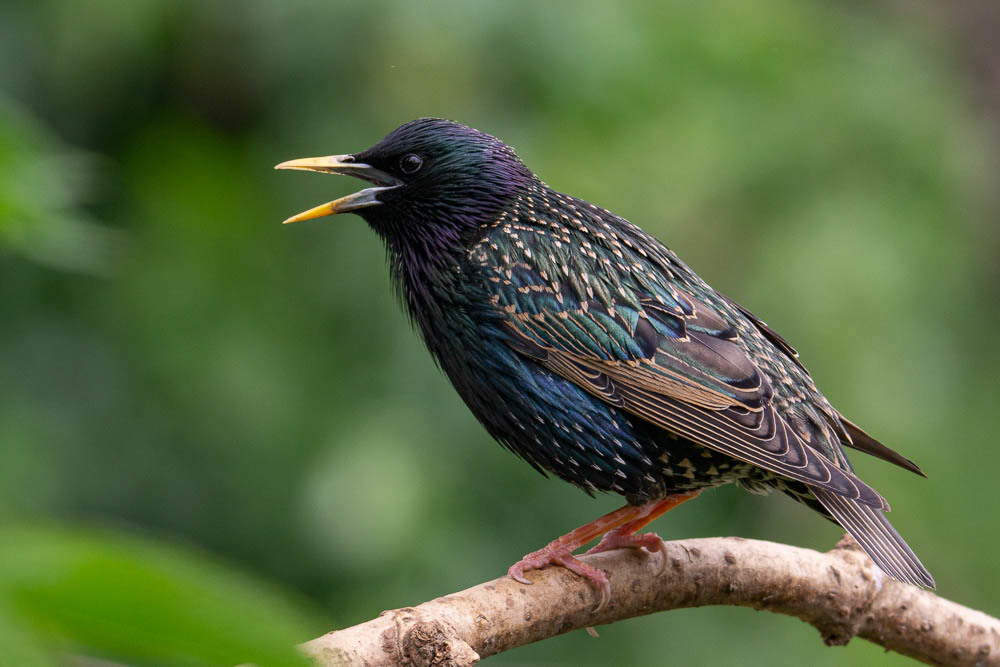
\includegraphics[width=0.6\textwidth]{Problem_5/Figs_P5/fig02.jpg}\caption{Một chú chim sáo đá châu Âu (\textit{Sturnus vulgaris}).}
    \label{fig:Sturn}
\end{figure}

\ \ 


\newpage

{\normalcolor\textbf{CÂU 6. (4.0 điểm)}}\vspace{1.5mm}

\setcounter{equation}{0}
Một chiếc khung có bao gồm 5 thanh cứng đồng chất khối lượng $m$ vài có chiều dài $l$ được nối với sàn và nối với nhau bằng các chốt tạo thành lục giác với các cạnh bằng nhau và nằm đối xứng 2 bên (như hình vẽ). Xem rằng không có các ma sát tại các chốt nối. Gọi góc $\alpha$ là góc tạo bởi một thanh ở bên với mặt phẳng nằm ngang. Gia tốc trọng trường là $g$.

\vspace{-3mm}
\begin{center}
\begin{minipage}{0.4\textwidth}
\hspace{0.15\textwidth}
    \begin{tikzpicture}
        %Sàn
        \draw (-2.5,0)--(2.5,0);
        \multiput(-2.5,0)(0.1,0){51}{\line(1,-3){0.12}}
        %Thanh
        \draw[very thick] (-1,0)--(-2,1.7)--(-1,3.4)--(1,3.4)--(2,1.7)--(1,0);
        %Khớp nối
        \filldraw[color=black, fill=ColorOr, ultra thick](-1,0) circle (0.1);
        \filldraw[color=black, fill=ColorOr, ultra thick](1,0) circle (0.1);
        \filldraw[color=black, fill=ColorOr, ultra thick](-2,1.7) circle (0.1);
        \filldraw[color=black, fill=ColorOr, ultra thick](2,1.7) circle (0.1);
        \filldraw[color=black, fill=ColorOr, ultra thick](-1,3.4) circle (0.1);
        \filldraw[color=black, fill=ColorOr, ultra thick](1,3.4) circle (0.1);
        %Ký hiệu
        \draw[->] (2.2,3.3)--(2.2,2.3);
        \draw (2.3,2.8) node[right]{$\vec{g}$};
        \draw (-1.2,0.3) arc (120:180:0.3);
        \draw (-1.8,0.2) node[right]{$\alpha$};
        \draw[thick,->] (0,3.4)--(0,4.4);
        \draw (0.1,3.9) node[right]{$\vec{F}$};
        \filldraw[color=white, fill=white, ultra thick](0,4.3) circle (0.1);
        \draw[<->] (-2.3,0)--(-2.3,3.4);
        \draw (-2.3,1.7) node[left]{$x$};
        \draw[thick,->] (0,3.4)--(0,4.4);
        \draw (0.1,3.9) node[right]{$\vec{F}$};
    \end{tikzpicture}
\end{minipage}    
\hspace{0.1\textwidth}
\begin{minipage}{0.4\textwidth}
    \begin{tikzpicture}
        %Sàn
        \draw (-2.5,0)--(2.5,0);
        \multiput(-2.5,0)(0.1,0){51}{\line(1,-3){0.12}}
        %Thanh
        \draw[very thick] (-1,0)--(-2,1.7)--(-1,3.4)--(1,3.4)--(2,1.7)--(1,0);
        %Khớp nối
        \filldraw[color=black, fill=ColorOr, ultra thick](-1,0) circle (0.1);
        \filldraw[color=black, fill=ColorOr, ultra thick](1,0) circle (0.1);
        \filldraw[color=black, fill=ColorOr, ultra thick](-2,1.7) circle (0.1);
        \filldraw[color=black, fill=ColorOr, ultra thick](2,1.7) circle (0.1);
        \filldraw[color=black, fill=ColorOr, ultra thick](-1,3.4) circle (0.1);
        \filldraw[color=black, fill=ColorOr, ultra thick](1,3.4) circle (0.1);
        %Ký hiệu
        \draw (-1.2,0.3) arc (120:180:0.3);
        \draw (-2.0,0.2) node[right]{$\alpha$};
        \filldraw[color=black, fill=gray, ultra thick](0,4.3) circle (0.1);
        \draw[thick,->] (0,4.3)--(0,3.5);
        \draw (0.1,4) node[right]{$\vec{v}_0$};
    \end{tikzpicture}
\end{minipage}    
\end{center}

\noindent \textbf{1.} Ta đặt vào tâm của thanh ở giữa một lực $F$ theo phương thẳng đừng hướng từ dưới lên trên. Xác định gia tốc góc các thanh $\ddot{\alpha}$ ở bên tại thời điểm cơ hệ đang đứng yên tạm thời ($\dot{\alpha}=0$) theo $m$, $g$, $F$ và $\alpha$. 

\noindent \textbf{2.} Xét trường hợp lực $F$ đặt vào giữa thanh ở giữa theo phương từ dưới lên trên và độ lớn có dạng $F=k(x_0-x)$ với $x$ là khoảng cách từ sàn tới độ cao của thanh ở giữa, $k$ và $x_0$ là các hằng số. Tại vị trí góc $\alpha=\alpha_0$, hệ khung đạt trạng thái cân bằng bền.
\begin{enumerate}[label=\textbf{\alph*,}]\itemsep0em
    \item Tìm hằng số $x_0$ theo $l$, $m$, $g$, $k$ và $\alpha_0$.
    \item Tính chu kỳ dao động nhỏ của hệ quanh vị trí cân bằng bền theo $l$, $m$, $g$, $k$ và $\alpha_0$.
\end{enumerate}
\noindent \textbf{3.} Bỏ qua lực $F$ đặt vào hệ ở các phần trước. Tại thời điểm $\alpha=\alpha_1$ và $\dot{\alpha}=0$, một vật nhỏ có khối lượng $M$ có vận tốc $v_0$ theo phương thẳng đứng chiều từ trên xuống dưới đập vào tâm thanh ở giữa. Xem rằng va chạm này là va chạm hoàn toàn đàn hồi và thời gian va chạm vô cùng ngắn sao cho tọa độ của các vật thay đổi không đáng kể trong quá trình va chạm.
\begin{enumerate}[label=\textbf{\alph*,}]\itemsep0em
    \item Tính vận tốc góc $\dot{\alpha}$ của các thanh ở hai bên ngay sau va chạm.
    \item Tính vận tốc $v$ của vật nhỏ ngay sau va chạm.
\end{enumerate}

\begin{flushright}
    (Biên soạn bởi Log)
\end{flushright}

{\normalcolor \textbf{CÂU 7. (4.0 điểm)}}\vspace{1.5mm}

\setcounter{equation}{0}
Có một sợi dây hình trụ bằng vật liệu đồng chất dẫn điện dẫn nhiệt, biết rằng khi nhiệt độ môi trường là $ T_{0} $ thì chiều dài của nó là $ l_{0} $, bán kính là $ r_{0} $ và điện trở suất của nó là $ \rho_{0} $.
Điện trở suất của vật liệu thay đổi theo nhiệt độ theo hàm $ \rho (T) = \rho_{0} \left (1+ \beta \left (T-T_{0} \right) \right) $, hệ số giãn nở tuyến tính là $\alpha$. Bây giờ một dòng điện có cường độ $ I $ chạy vào và đợi cho hệ cân bằng nhiệt. Biết rằng theo vật liệu toả nhiệt ra môi trường với hệ số $\lambda$ với công suất
$$\left(\frac{dQ}{dt}\right)_{\text{loss}} = \lambda S (T - T_0),$$




\begin{minipage}{0.76\textwidth}
với $S$ là diện tích bề mặt toả nhiệt.

\begin{enumerate}[label=\textbf{\alph*,}]\itemsep0em
\item Giả sử rằng hình trụ dẫn nhiệt tốt và nhiệt độ tại mỗi vị trí là như nhau khi nó ổn định, hãy tính nhiệt độ $ T_{f} $ lúc cân bằng (khai triển đến bậc nhất của $\alpha$, $\beta$).
\item Giả sử rằng hình trụ dài và nhiệt độ khác nhau tại các vị trí khác nhau trong quá trình cân bằng, điện trở suất và sự nở vì nhiệt được bỏ qua (nghĩa là lấy $ \alpha = \beta = 0 $), hệ số dẫn nhiệt Fourier $ k $ là một hằng số và nhiệt độ ở cả hai đầu được giả định là $ T_{0} $, hãy tìm phân bố nhiệt độ $ T (x) $ trên khối trụ. 
\end{enumerate}
\end{minipage}
\begin{minipage}{0.35\textwidth}
\quad \quad
  \begin{tikzpicture}[scale=0.85]
\draw[dashed](0,1.5,0)--(0,-1.5,0);
\draw[thick,-stealth](0,-3)--(0,-1.5);
    \draw[dashed] (1.5,0) arc (0:180:1.5cm and 0.6cm);
    \draw[dashed] (1.5,-1.5) arc (0:180:1.5cm and 0.5cm);
	\shade[shading=radial, inner color=orange!20!white, outer color=orange!60!white, opacity=0.70] (1.5,1.5) -- (1.5,-1.5) arc (360:180:1.5cm and 0.5cm) -- (-1.5,1.5) arc (180:360:1.5cm and 0.5cm) ;
	\draw[] (1.5,1.5) -- (1.5,-1.5) arc (360:180:1.5cm and 0.5cm) -- (-1.5,1.5) arc (180:360:1.5cm and 0.5cm) ;
  \draw[dashed] (1.5,0) arc (360:180:1.5cm and 0.6cm);
  \shade[shading=radial, inner color=orange!20!white, outer color=orange!60!white, opacity=0.70] (1.5,1.5) arc (0:360:1.5cm and 0.5cm); 
  \draw (1.5,1.5) arc (0:360:1.5cm and 0.5cm);
  \draw [dashed] (0,1.5)--(1.5,1.5);
	\node at (0.8,1.7) {$r_0$};
\draw[thick,-stealth](0,1.5)--(0,3);
\draw (0,-2.5) node[right]{$I$};
\draw (0,2.5) node[right]{$I$};
\end{tikzpicture}	
\end{minipage}

\vspace{1.5mm}
\textit{Gợi ý: Nghiệm tổng quát của phương trình vi phân tuyến tính thuần nhất $ y ^{\prime \prime} -A y + B = 0$ $(A> 0) $ là} 
$$ y = \cfrac{B}{A} + C_{1} e ^{ \sqrt{A} x} + C_{2} e ^{- \sqrt{A} x} ,$$
\textit{với $C_1$ và $C_2$ là các hằng số được xác định từ các điều kiện ban đầu.}

\begin{flushright}
    (Biên soạn bởi Zinc và Yukon)
\end{flushright}

{\normalcolor \textbf{CÂU 8. (4.0 điểm)}}\vspace{1.5mm}

\setcounter{equation}{0}
Máy co góc plasma (\textit{Angular pinch}) sử dụng từ trường để tăng tốc và định hướng dòng plasma, do đó nó có thể tạo ra một vụ nổ plasma tại một mục tiêu ngay lập tức. Thiết bị được thể hiện trên hình dưới. Có một tấm dẫn xung quanh ống thủy tinh chân không và chứa một thanh mục tiêu có cùng chiều dài, bỏ qua độ dày của thành ống thủy tinh và độ dày của vỏ ruột dẫn, và $ H \gg R_{ 2} $. Ống chứa đầy hiđro bị ion hóa thành plasma có mật độ số điện tích dương và âm đều là $n$. Khi $ t = 0 $, người ta đặt một nguồn điện vào vỏ dây dẫn để dòng điện tăng nhanh từ 0 đến $ I $ và dòng điện $ I $ được giữ nguyên trong một khoảng thời gian, dòng điện chạy đều dọc theo hướng tiếp tuyến của vỏ hình trụ. Bỏ qua chuyển động nhiệt của các hạt, tương tác Coulomb và va chạm giữa các hạt, điện tích nguyên tố là $ e $, khối lượng của các electron và hạt nhân hydro lần lượt là $ m_{e}, m_{p} $.

\begin{figure}[!htb]
    \centering
    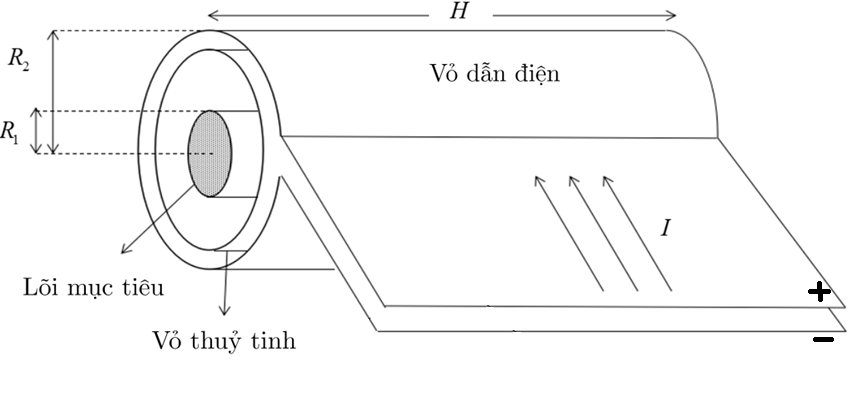
\includegraphics[scale=0.55]{Problem_8/P8.png}
    \label{fig_P8}
\end{figure}
\begin{enumerate}[label=\textbf{\alph*,}]\itemsep0em
\item Một hạt có điện tích $ q $ và khối lượng $ m $ ở khoảng cách từ trục trung tâm $ r \left (R_{1} <r <R_{2} \right) $ sau khi dòng điện ổn định tới $ I $. Tìm tốc độ tức thời $ v_{0} $ của hạt.    
    \item Tìm thời điểm $ t (r) $ khi hạt trong câu hỏi trước chuyển động đến vị trí $ R_{1} $.
    \item Giả sử hạt va chạm với thanh mục tiêu hoàn toàn không đàn hồi, tìm áp suất $ P (t) $ trên bề mặt của thanh mục tiêu tại thời điểm $ t $. Trên thực tế, plasma trong ống là các electron và hạt nhân hydro bị ion hóa, điều này cho thấy chuyển động của một loại hạt có thể bị bỏ qua khi $ t $ nhỏ, và ảnh hưởng của hạt này cần được bỏ qua trong câu trả lời cuối cùng.
    \item Xác định thông số thiết bị $ \beta = \cfrac {P_{\max}} {\omega_{B}} $, trong đó $ \omega_{B} $ là mật độ năng lượng của từ trường chân không và độ lớn của nó là $ \cfrac {B^{2}} {2 \mu_{0}} $. Sau đó, so sánh nó với $ \beta \left(\approx 10^{-1} \sim 1 \right) $ của hầu hết các thiết bị Tokamak (định hướng dòng plasma dạng donut) và thể hiện những ưu điểm của máy co góc. Đối với phép tính số trong câu hỏi này, hãy thay $\cfrac{\mu_{0}}{4 \pi} = 1 \times 10^{- 7} \mathrm {~N} / \mathrm {A}^{2}$, $H = 30.0 \mathrm {~m}$, $R_{1} = 1.0 \mathrm{~mm}$, $R_{2} = 1.00 \mathrm{~m}$, $n = 1.00 \times 10^{8} \mathrm {~m}^{-3}$.
\end{enumerate}

\begin{flushright}
    (Biên soạn bởi Zinc và Yukon)
\end{flushright}

{\normalcolor\textbf{CÂU 9. (4.0 điểm)}}\vspace{1.5mm}

\setcounter{equation}{0}
\textbf{Bức xạ vùng xa}

Trong truyền sóng điện từ không dây, "trường xa" thường được hiểu là trường điện từ ở vị trí xa nguồn phát $r$ hơn nhiều lần bước sóng điện từ $\lambda$. Khi khảo sát ảnh hưởng của trường điện từ tại vùng không gian này, hiện tượng cảm ứng điện từ chiếm ưu thế hoàn toàn so với điện từ trường như trong các mô hình tĩnh điện (định luật Coulomb) hay từ dừng (định luật Bio-Savart-Laplace).

\begin{center}
\begin{minipage}{\textwidth}
\centering
\begin{tikzpicture}[scale=0.8]
    %%Decartes_coordinate
    \draw[-Stealth] (0,0) to (0,5);
    \draw[-Stealth] (0,0) to (5,0);
    \draw[-Stealth] (0,0) to (-4,-3);
    \draw[fill=black] (0,0) circle (0.05);
    \draw 
    (4.5,0) node[above]{$y$}
    (0,4.5) node[left]{$z$}
    (-3.6,-2.6) node[left]{$x$};
    %%Sphere_coordinate
    \draw (0,0) circle (4);
    \draw (0,4) arc(90:-90:2 and 4);
    \draw[dashed] (0,4) arc(90:270:2 and 4);
    \draw (-4,0) arc(180:360:4 and 2);
    \draw[dashed] (4,0) arc(0:180:4 and 2);
    %%projection
    \draw[fill=black] (1.4,2.85) circle (0.05);
    \draw (0,0) to (1.4,2.85) to (1.4,-1.4) to (0,0);
    \draw[dashed] (1.4,-1.4) to (1.75,-1.75);
    \draw[-Stealth] (-0.8,-0.6) arc(-130:-45:1);
    \draw[-Stealth] (0,1) arc(90:63:1);
    \draw 
    (-0.3,-1.2) node{$\phi$}
    (0.25,1.4) node{$\theta$}
    (0.9,1.2) node{$r$};
    %%unit vector
    \draw[-Stealth] (1.4,2.85) to (2,4.1);
    \draw[-Stealth] (1.4,2.85) to (2,1.7);
    \draw[-Stealth] (1.4,2.85) to (2.5,3.3);
    \draw
    (2.2,2.8) node{$\hat{\phi}$}
    (2.1,2.2) node{$\hat{\theta}$}
    (1.5,4) node{$\hat{r}$};
    %%antenna
    \draw[ultra thick, -Stealth] (0,-0.5) to (0,0.5);
    \draw (-0.6,0.1) node{$I,\delta$};
\end{tikzpicture}
\end{minipage} \\
\vspace{2mm} 
Hình 1: Hệ tọa độ cầu và vị trí của dây dẫn.
\end{center}

Theo đó, một đoạn dây dẫn vô cùng ngắn có chiều dài $\delta \ll \lambda$ có dòng điện xoay chiều $I = I_0 \cos \omega t$ chạy qua và tích điện hai đầu dây như một lưỡng cực điện sẽ giống như một nguồn phát sóng điện từ có dạng
\begin{equation*}
    \Vec{E} = - \omega \mu \dfrac{I_0 \delta}{4 \pi r} \sin \left( \omega t - \dfrac{2 \pi r}{\lambda} \right) \sin \theta \hat{\theta}.
\end{equation*}
Và cường độ từ trường
\begin{equation*}
    \Vec{H} = - \omega \sqrt{\mu \varepsilon} \dfrac{I_0 \delta}{4 \pi r} \sin \left( \omega t - \dfrac{2 \pi r}{\lambda} \right) \sin \theta \hat{\phi}.
\end{equation*}

Năng lượng bức xạ của sóng điện từ qua một đơn vị diện tích trong một đơn vị thời gian được biểu diễn qua vector Poynting theo biểu thức
\begin{equation*}
    \Vec{S} = \Vec{E} \times \Vec{H}.
\end{equation*}

\begin{enumerate}
    \item Xét một đoạn dây thẳng có độ dài $l_1 \ll \lambda$ có dòng $I=I_0 \cos \omega t$. 
    \begin{enumerate}
        \item Hãy tìm công suất bức xạ trung bình $P$ của đoạn dây.
        \item Công suất phát xạ sóng điện từ của đoạn dây tiêu hao năng lượng tương đương một thành phần điện trở $R_r$. Hãy xác định điện trở $R_r$.
    \end{enumerate}
    \item Xét một đoạn dây thẳng có độ dài $l_2$ so sánh được với $\lambda$ và có dòng điện $I=I_0 \cos \omega t$ chạy qua. Xét các điểm cùng cách tâm đoạn dây thẳng một khoảng $r$, tìm tỷ số cường độ sóng truyền theo phương hợp với dây một góc $\theta$ và cường độ sóng truyền theo phương $\theta=\pi/2$.
\end{enumerate}

\begin{flushright}
    (Biên soạn bởi Log)
\end{flushright}

{\normalcolor\textbf{CÂU 10. (4.0 điểm)}}\vspace{1.5mm}

\setcounter{equation}{0}
\textbf{Tâm sai quỹ đạo trái đất} \\
Quỹ đạo Trái Đất quanh Mặt Trời không phải là một hình tròn hoàn hảo mà là một hình ellipse với tâm sai \(\varepsilon\). Chính vì vậy, thời gian giữa các sự kiện Xuân phân, Hạ chí, Thu phân và Đông chí là không đều nhau. Trong bài tập này, chúng ta sẽ đưa ra một mô hình tính toán tâm sai của trái đất với sai số cỡ $9 \%$ thông qua các thông tin về những ngày đặc biệt trong năm (như bảng dưới). \\
% Một số thông tin cơ bản về hình ellipse: %(em cần ký hiệu bán trục lớn, nhỏ, bán tiêu cự, trục x, y, r và góc của 1 điểm bất kỳ)
% \(a\): Bán trục lớn \\
% \(b\): Bán trục nhỏ \\
% \(c\): Bán tiêu cự \\
% \(\varepsilon\): Tâm sai \\
% Công thức tâm sai:
% \begin{equation*}
%     \varepsilon = \frac{c}{a} = \sqrt{1 - \frac{b^2}{a^2}}
% \end{equation*}
% Phương trình ellipse trong hệ tọa độ Descartes: 
% \begin{equation*}
%     \frac{x^2}{a^2} + \frac{y^2}{b^2} = 1 
% \end{equation*}
% Phương trình ellipse trong hệ tọa độ cực: 
% \begin{equation*}
%     r = \frac{a(1-e^2)}{1 - \varepsilon \cos{\phi}}
% \end{equation*}
\vspace{-0.5cm}
\begin{center}
\footnotesize{
\begin{tabular}{|>{\centering\arraybackslash}m{4cm}|>{\centering\arraybackslash}m{4cm}|>{\centering\arraybackslash}m{3cm}|>{\centering\arraybackslash}m{3cm}|}
    \hline
    Sự kiện & Thời điểm & Thời gian kể từ sự kiện trước (ngày) & Số ngày trôi qua \\
    \hline
    Xuân phân 2022 (VE) & 20/03/2022, 15h33 & - & - \\
    \hline
    Hạ chí 2022 (SS) & 21/06/2022, 09h14 & 92.7368 & 93 \\
    \hline
    Thu phân 2022 (AE) & 23/09/2022, 01h04 & 93.6597 & 93 \\
    \hline
    Đông chí 2022 (WS) & 21/12/2022, 21h48 & 89.8939 & 90 \\
    \hline
    Xuân phân 2023 (VE) & 20/03/2023, 21h24 & 88.9833 & 89 \\
    \hline
\end{tabular} }
\end{center}
\begin{enumerate}[label=\textbf{\arabic*,}]\itemsep0em 
        \item \textbf{Định luật 2 Kepler} \\
        Biểu diễn vận tốc quét \(dS/dt\) theo moment động lượng của Trái Đất \(L_E\) và khối lượng Trái Đất \(m_E\), trong đó \(S\) là diện tích quét được của đường nối Mặt Trời và Trái Đất. Từ đó kiểm nghiệm lại quan sát của Kepler: Diện tích quét được của đường nối hành tinh và Mặt Trời là như nhau trong khoảng thời gian bằng nhau.
        \item \textbf{Xác định tâm sai quỹ đạo Trái Đất}
\vspace{-0.8cm}
\begin{center}
\begin{minipage}{\textwidth}
\centering
\begin{tikzpicture}[scale=0.8]
    \draw[thick] (0,0) ellipse (4 and 2.5);
    \draw[thick, gray] (-8,0) to (8,0);
    \draw[fill=red!60, thick] (-1,0) circle (0.25);
    \draw[dashed, thick, gray] 
    (-4.5,-1.17) to (4.5,1.83)
    (0,-3) to (-2,3);
    \draw[thick, magenta, -Stealth] (-0.4,0) arc (0:290:0.6);
    \draw 
    (-6,0) node[above]{Điểm cận nhật} 
    (6,0) node[below]{Điểm viễn nhật}
    (-1.8,0.7) node{$\phi_{VE}$}
    (-5,-1.4) node{WS}
    (4.8,2) node{SS}
    (-2,3) node[above]{AE}
    (0,-3) node[below]{VE};
\end{tikzpicture}
\end{minipage} \\
\vspace{2mm}
Hình 1: Vị trí bốn sự kiện đặc biệt trong năm.
\end{center}
% \vspace{-0.5cm}
Kí hiệu \(\phi_1\), \(\phi_2\) (\(\phi_2 > \phi_1\)) là góc lượng giác hợp bởi điểm viễn nhật và 2 điểm 1, 2 bất kỳ trên quỹ đạo. Thời gian đi từ 1 đến 2 \(t_{1 \rightarrow 2}\) được cho bởi tích phân sau:
\begin{equation*}
    t_{1 \rightarrow 2} = A \int_{\phi_1}^{\phi_2} \frac{d\phi}{(1-\varepsilon \cos{\phi})^2}.
\end{equation*}
\textbf{a,} Biểu diễn \(A\) theo chu kỳ \(T\) và tâm sai \(\varepsilon\) của trái đất. \\
\textbf{b,} Tâm sai quỹ đạo Trái Đất là nhỏ. Từ phương trình đề bài cho, hãy rút ra xấp xỉ sau:
\begin{equation*}
    t_{1 \rightarrow 2} \approx A[(\phi_2 - \phi_1) + 2\varepsilon(\sin{\phi_2} - \sin{\phi_1})].
\end{equation*}
\textbf{c,} Sử dụng các số liệu cho trong bảng, xử lý và đưa ra tâm sai của quỹ đạo Trái Đất \(\varepsilon\).
\end{enumerate}

\begin{flushright}
    (Biên soạn bởi manhducnmd và Log)
\end{flushright}



\begin{center}
    \normalcolor{------------------------------------------------ HẾT ------------------------------------------------}
\end{center}

\end{document}